\documentclass{amsart}

%auto-ignore
%this ensures the arxiv doesn't try to start TeXing here.
%!TEX root=trivalent.tex

\usepackage{amsmath,amssymb,amsfonts,amsthm}
\usepackage{ifpdf}
\usepackage{enumerate}
\usepackage{ulem}
\usepackage{leftidx}

\usepackage{breqn}

\usepackage{tikz}
\usetikzlibrary{calc}
\usepackage{tikz-qtree}


\ifpdf
\usepackage[pdftex,plainpages=false,hypertexnames=false,pdfpagelabels]{hyperref}
\else
\usepackage[dvips,plainpages=false,hypertexnames=false]{hyperref}
\fi


% ----------------------------------------------------------------
\vfuzz2pt % Don't report over-full v-boxes if over-edge is small
\hfuzz2pt % Don't report over-full h-boxes if over-edge is small
% ----------------------------------------------------------------

% diagrams -------------------------------------------------------
% figures ---------------------------------------------------------
%%% borrowed from Dror's cobordisms paper, use this to include eps or pdf graphics.
\newcommand{\pathtodiagrams}{diagrams/pdf/}

\newcommand{\mathfig}[2]{{\hspace{-3pt}\begin{array}{c}%
  \raisebox{-2.5pt}{\includegraphics[width=#1\textwidth]{\pathtodiagrams #2}}%
\end{array}\hspace{-3pt}}}

\newcommand{\inputtikz}[1]{\input{diagrams/tikz/#1.tex}}

\newcommand{\arxiv}[1]{\href{http://arxiv.org/abs/#1}{\tt arXiv:\nolinkurl{#1}}}
\newcommand{\doi}[1]{\href{http://dx.doi.org/#1}{{\tt DOI:#1}}}
\newcommand{\euclid}[1]{\href{http://projecteuclid.org/getRecord?id=#1}{{\tt #1}}}
\newcommand{\mathscinet}[1]{\href{http://www.ams.org/mathscinet-getitem?mr=#1}{\tt #1}}
\newcommand{\googlebooks}[1]{(preview at \href{http://books.google.com/books?id=#1}{google books})}

% THEOREMS -------------------------------------------------------
\theoremstyle{plain}
%\newtheorem*{fact}{Fact}
\newtheorem{prop}{Proposition}[section]
\newtheorem{conj}[prop]{Conjecture}
\newtheorem{thm}[prop]{Theorem}
\newtheorem{recipe}[prop]{Recipe}
\newtheorem{lem}[prop]{Lemma}
\newtheorem{alg}[prop]{Algorithm}
\newtheorem{cor}[prop]{Corollary}
\newtheorem*{cor*}{Corollary}
%\newtheorem*{example}{Example}
\newtheorem{question}{Question}
\newtheorem*{kuperberg}{The Kuperberg Program}
\newenvironment{rem}{\\ \noindent\textsl{Remark.}}{}  % perhaps looks better than rem above?
\numberwithin{equation}{section}
%\numberwithin{figure}{section}

\theoremstyle{remark}
\newtheorem{ex}[prop]{Example}
\newtheorem*{exc}{Exercise}
\newtheorem{remark}[prop]{Remark}           
\newtheorem*{rem*}{Remark}               %unnumbered remark
\newtheorem*{ex*}{Example}                %unnumbered exercise

\theoremstyle{definition}
\newtheorem{defn}[prop]{Definition}         % numbered definition
\newtheorem{assumption}[prop]{Assumption}   
\newtheorem{nota}[prop]{Notation}   
\newtheorem*{defn*}{Definition}             % unnumbered definition


\theoremstyle{plain}
\newcommand{\noqed}{\renewcommand{\qedsymbol}{}}

% Marginal notes in draft mode -----------------------------------
\newcommand{\scott}[1]{\stepcounter{comment}{{\color{green} $\star^{(\arabic{comment})}$}}\marginpar{\color{green}  $\star^{(\arabic{comment})}$ \usefont{T1}{scott}{m}{n}  #1 --S}}     % draft mode
\newcommand{\eep}[1]{\stepcounter{comment}{\color{blue} $\star^{(\arabic{comment})}$}\marginpar{\color{blue}  $\star^{(\arabic{comment})}$  #1 --E}}     % draft mode
\newcommand{\comment}[1]{\stepcounter{comment}$\star^{(\arabic{comment})}$\marginpar{\tiny $\star^{(\arabic{comment})}$ #1}}     % draft mode
\newcounter{comment}
\newcommand{\noop}[1]{}
\newcommand{\todo}[1]{\textcolor{blue}{\textbf{TODO: #1}}}
\newcommand{\nn}[1]{\textcolor{red}{[[#1]]}}

% \mathrlap -- a horizontal \smash--------------------------------
% For comparison, the existing overlap macros:
% \def\llap#1{\hbox to 0pt{\hss#1}}
% \def\rlap#1{\hbox to 0pt{#1\hss}}
\def\clap#1{\hbox to 0pt{\hss#1\hss}}
\def\mathllap{\mathpalette\mathllapinternal}
\def\mathrlap{\mathpalette\mathrlapinternal}
\def\mathclap{\mathpalette\mathclapinternal}
\def\mathllapinternal#1#2{%
\llap{$\mathsurround=0pt#1{#2}$}}
\def\mathrlapinternal#1#2{%
\rlap{$\mathsurround=0pt#1{#2}$}}
\def\mathclapinternal#1#2{%
\clap{$\mathsurround=0pt#1{#2}$}}

% MATH -----------------------------------------------------------
\newcommand{\Natural}{\mathbb N}
\newcommand{\Integer}{\mathbb Z}
\newcommand{\Rational}{\mathbb Q}
\newcommand{\Real}{\mathbb R}
\newcommand{\Complex}{\mathbb C}
\newcommand{\Field}{\mathbb F}

% tricky way to iterate macros over a list
\def\semicolon{;}
\def\applytolist#1{
    \expandafter\def\csname multi#1\endcsname##1{
        \def\multiack{##1}\ifx\multiack\semicolon
            \def\next{\relax}
        \else
            \csname #1\endcsname{##1}
            \def\next{\csname multi#1\endcsname}
        \fi
        \next}
    \csname multi#1\endcsname}

% \def\cA{{\cal A}} for A..Z
\def\calc#1{\expandafter\def\csname c#1\endcsname{{\mathcal #1}}}
\applytolist{calc}QWERTYUIOPLKJHGFDSAZXCVBNM;
% \def\bbA{{\mathbb A}} for A..Z
\def\bbc#1{\expandafter\def\csname bb#1\endcsname{{\mathbb #1}}}
\applytolist{bbc}QWERTYUIOPLKJHGFDSAZXCVBNM;
% \def\bfA{{\mathbf A}} for A..Z
\def\bfc#1{\expandafter\def\csname bf#1\endcsname{{\mathbf #1}}}
\applytolist{bfc}QWERTYUIOPLKJHGFDSAZXCVBNM;


\newcommand{\id}{\boldsymbol{1}}
\renewcommand{\imath}{\mathfrak{i}}
\renewcommand{\jmath}{\mathfrak{j}}

\newcommand{\qRing}{\Integer[q,q^{-1}]}
\newcommand{\qMod}{\qRing-\operatorname{Mod}}
\newcommand{\ZMod}{\Integer-\operatorname{Mod}}

\newcommand{\into}{\hookrightarrow}
\newcommand{\onto}{\twoheadrightarrow}
\newcommand{\iso}{\cong}
\newcommand{\actsOn}{\circlearrowright}

\newcommand{\htpy}{\simeq}

\newcommand{\abs}[1]{\left|#1\right|}
\newcommand{\norm}[1]{\left|\left|#1\right|\right|}
\newcommand{\ip}[1]{\left< #1\right>}

\newcommand{\restrict}[2]{#1{}_{\mid #2}{}}
\newcommand{\set}[1]{\left\{#1\right\}}
\newcommand{\setc}[2]{\left\{#1 \;\left| \; #2 \right. \right\}}
\newcommand{\quotient}[2]{\frac{#1}{#2}}
\newcommand{\relations}[2]{\left<#1 \;\left| \; #2 \right. \right>}
\newcommand{\cone}[3]{C\left(#1 \xrightarrow{#2} #3\right)}
\newcommand{\pairing}[2]{\left\langle#1 ,#2 \right\rangle}

\newcommand{\code}[1]{{\tt #1}}
\newcommand{\MMA}{\code{Mathematica} {}}

\newcommand{\bigraph}[1]{{\hspace{-3pt}\begin{array}{c}%
  \raisebox{-2.5pt}{\includegraphics[height=6mm]{\pathtographs \hashlookup{#1}}}% 
\end{array}\hspace{-3pt}}}

\newcommand{\graph}[1]{{\hspace{-3pt}\begin{array}{c}%
  \raisebox{-2.5pt}{\includegraphics[height=10mm]{\pathtographs \hashlookup{#1}}}% 
\end{array}\hspace{-3pt}}}

\newcommand{\J}[2]{\mathcal{J}_{#1,#2}}
\newcommand{\Jf}[2]{\mathcal{J}^{\text{framed}}_{#1,#2}}
\newcommand{\HOMFLY}{\operatorname{HOMFLYPT}}
\newcommand{\Kauffman}{\operatorname{Kauffman}}
\newcommand{\Dubrovnik}{\operatorname{Dubrovnik}}
\newcommand{\Rep}{\operatorname{Rep}}
\newcommand{\vRep}{\Rep^{\text{vector}}}

\newcommand{\overcrossing}{\inputtikz{overcrossing}}
\newcommand{\undercrossing}{\inputtikz{undercrossing}}
\newcommand{\identity}{\inputtikz{identity}}
\newcommand{\cupcap}{\inputtikz{cupcap}}
\newcommand{\Oovercrossing}{\inputtikz{Oovercrossing}}
\newcommand{\Oundercrossing}{\inputtikz{Oundercrossing}}
\newcommand{\Oidentity}{\inputtikz{Oidentity}}

\newcommand{\positivetwist}{\inputtikz{positivetwist}}
\newcommand{\negativetwist}{\inputtikz{negativetwist}}
\newcommand{\verticalstrand}{\inputtikz{verticalstrand}}

\newcommand{\card}[1]{\sharp{#1}}

\newcommand{\bdy}{\partial}
\newcommand{\compose}{\circ}
\newcommand{\eset}{\emptyset}
\newcommand{\disj}{\sqcup}

\newcommand{\psmallmatrix}[1]{\left(\begin{smallmatrix} #1 \end{smallmatrix}\right)}

\newcommand{\qiq}[2]{[#1]_{#2}}
\newcommand{\qi}[1]{\qiq{#1}{q}}
\newcommand{\qdim}{\operatorname{dim_q}}

\newcommand{\directSum}{\oplus}
\newcommand{\DirectSum}{\bigoplus}
\newcommand{\tensor}{\otimes}
\newcommand{\Tensor}{\bigotimes}

\newcommand{\altTensor}{\widehat{\Tensor}}

\newcommand{\db}[1]{\left(\left(#1\right)\right)}

\newcommand{\su}[1]{\mathfrak{su}_{#1}}
\newcommand{\csl}[1]{\mathfrak{sl}_{#1}}
\newcommand{\uqsl}[1]{U_q\left(\csl{#1}\right)}

\newcommand{\Cobl}{{\mathcal Cob}_{/l}}
\newcommand{\Cob}[1]{{\mathcal Cob}\left(\su{#1}\right)}
\newcommand{\Kom}[1]{\operatorname{Kom}\left(#1\right)}

\newcommand{\Mat}[1]{\operatorname{\mathbf{Mat}}\left(#1\right)}
\newcommand{\Inv}[1]{\operatorname{Inv}\left(#1\right)}
\newcommand{\Hom}{\operatorname{Hom}}
\newcommand{\End}[1]{\operatorname{End}\left(#1\right)}
\newcommand{\Reigenvalue}[2]{R_{#1 \subset #2 \tensor #2}}
\newcommand{\tildeReigenvalue}[2]{\tilde{R}_{#1 \subset #2 \tensor #2}}
\newcommand{\im}{\operatorname{im}}

\newcommand{\lk}[2]{\operatorname{lk}\left(#1,#2\right)}
\newcommand{\fr}[1]{\operatorname{fr}\left(#1\right)}

\newcommand{\asbimod}[2]{\operatorname{Mod}'\left(#1 \subset #2\right)}
\newcommand{\sbimod}[2]{\operatorname{Mod}\left(#1 \subset #2\right)}
\newcommand{\abimod}[2]{#1-\operatorname{Mod}'-#2}
\newcommand{\bimod}[2]{#1-\operatorname{Mod}-#2}
\newcommand{\bimodule}[3]{\leftidx{_#1}{#2}{_#3}}

\newcommand{\pa}{\mathcal{PA}}
\newcommand{\TL}{\mathcal{TL}}
\newcommand{\JW}[1]{f^{(#1)}}
\newcommand{\tr}[1]{\text{tr}(#1)}
\newcommand{\dn}[1]{{\mathcal D}{\mathit (#1)}}

\newcommand{\directSumStack}[2]{{\begin{matrix}#1 \\ \DirectSum \\#2\end{matrix}}}
\newcommand{\directSumStackThree}[3]{{\begin{matrix}#1 \\ \DirectSum \\#2 \\ \DirectSum \\#3\end{matrix}}}

\newcommand{\grading}[1]{{\color{blue}\{#1\}}}
\newcommand{\shift}[1]{\left[#1\right]}

\newcommand{\tensorover}[1]{\otimes_{#1}}
\newcommand{\tensorhat}{\widehat{\Tensor}}

\newcommand{\LL}{\mathcal{L}}
\newcommand{\Lhat}{\hat{\mathcal{L}}}
\newcommand{\writhe}{\operatorname{writhe}}

\newenvironment{narrow}[2]{%
\vspace{-0.4cm}% horrible hack, by scott % this only seems to be appropriate in beamer mode...
\begin{list}{}{%
\setlength{\topsep}{0pt}%
\setlength{\leftmargin}{#1}%
\setlength{\rightmargin}{#2}%
\setlength{\listparindent}{\parindent}%
\setlength{\itemindent}{\parindent}%
\setlength{\parsep}{\parskip}}%
\item[]}{\end{list}}


%%% futzing with margins following Dror (from Karoubi)
%\marginparwidth 0pt%
%\marginparsep 0pt

\textwidth   5.5in%
\textheight  9.0in%
\oddsidemargin 12pt%
\evensidemargin 12pt

\topmargin -.6in%
\headsep .5in
% ----------------------------------------------------------------

\usepackage{tikz}
\usepackage{microtype}


\title{Categories generated by a trivalent vertex II}

\newcommand{\Cube}{\prism[45]{4}}
\newcommand{\PentPrism}{\prism{5}}
\newcommand{\HexPrism}{\prism{6}}
\newcommand{\Q}{
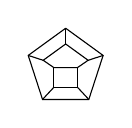
\begin{tikzpicture}[scale=.5]
	\draw (90:1cm)--(162:1cm)--(234:1cm)--(306:1cm)--(18:1cm)--(90:1cm);
	\draw (90:.6cm)--(162:.6cm)--(-.3,0)--(.3,0)--(18:.6cm)--(90:.6cm);
	\draw (18:.6cm)--(18:1cm);
	\draw (90:.6cm)--(90:1cm);
	\draw (162:.6cm)--(162:1cm);
	\draw (234:1cm) -- (-.3,-.5);
	\draw (306:1cm) -- (.3,-.5);
%	\draw (18:1cm)--(.3,0);
%	\draw (162:1cm)--(-.3,0);
	\draw (.3,0)--(-.3,0)--(-.3,-.5)--(.3,-.5)--(.3,0);
\end{tikzpicture}
}

\newcommand{\prism}[2][0]{
\begin{tikzpicture}[scale=0.8,baseline=-0.1cm]
\fill[white] (0,0) circle (0.5cm);
\foreach \x in {1, ..., #2} {
	\draw (360*\x/#2-360/#2+#1:.3cm) -- (360*\x/#2+#1:.3cm)--(360*\x/#2+#1:.5cm) -- (360*\x/#2+360/#2+#1:.5cm);
}
\end{tikzpicture}
}

%Draws an n-gon face with 120 degree angles.  the optional first argument is a rotation.
\newcommand{\ngon}[2][0]{
\begin{tikzpicture}[baseline=0cm]
\foreach \x in {1, ..., #2}
	\draw (360*\x/#2+#1:.8cm)--(360*\x/#2+#1:.5cm);
\foreach \x in {1, ..., #2}
	\draw (360*\x/#2+#1:.5cm) .. controls +(360*\x/#2+120+#1:.3cm) and +(360*\x/#2+360/#2-120+#1:.3cm) .. (360*\x/#2+360/#2+#1:.5cm);
\end{tikzpicture}
}

\newcommand{\drawI}{ 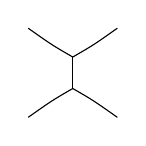
\begin{tikzpicture}[baseline=0cm]
 	\draw (0,.2) .. controls +(30:.3cm) .. (45:.8cm);
 	\draw (0,.2) .. controls +(150:.3cm) .. (135:.8cm);
	\draw (0,.2) -- (0,-.2);
 	\draw (0,-.2) .. controls +(-30:.3cm) .. (-45:.8cm);
 	\draw (0,-.2) .. controls +(-150:.3cm) .. (-135:.8cm);
\end{tikzpicture}
}

\newcommand{\drawH}{ 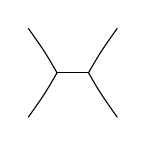
\begin{tikzpicture}[baseline=0cm,rotate=90]
 	\draw (0,.2) .. controls +(30:.3cm) .. (45:.8cm);
 	\draw (0,.2) .. controls +(150:.3cm) .. (135:.8cm);
	\draw (0,.2) -- (0,-.2);
 	\draw (0,-.2) .. controls +(-30:.3cm) .. (-45:.8cm);
 	\draw (0,-.2) .. controls +(-150:.3cm) .. (-135:.8cm);
\end{tikzpicture}}

\newcommand{\twostrandid}{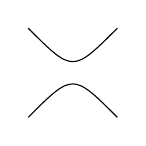
\begin{tikzpicture}[baseline=0cm]
	\draw (45:.8cm) .. controls (0,0) .. (135:.8cm);
	\draw (-45:.8cm) .. controls (0,0) .. (-135:.8cm);
\end{tikzpicture}}

\renewcommand{\cupcap}{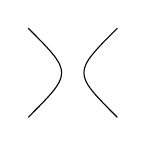
\begin{tikzpicture}[baseline=0cm,rotate=90]
	\draw (45:.8cm) .. controls (0,0) .. (135:.8cm);
	\draw (-45:.8cm) .. controls (0,0) .. (-135:.8cm);
\end{tikzpicture}}

\newcommand{\pentagon}{
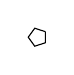
\begin{tikzpicture}[scale=.12,baseline=-2]
\draw (36:1) -- (108:1) -- (180:1) -- (252:1) -- (-36:1) -- (36:1);
\end{tikzpicture}
}

\newcommand{\psq}{
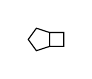
\begin{tikzpicture}[scale=.15,baseline=-2]
\draw (36:1) -- (108:1) -- (180:1) -- (252:1) -- (-36:1) -- (36:1) -- +(1.2,0) -- ($(-36:1)+(1.2,0)$) -- (-36:1);
\end{tikzpicture}
}

\newcommand{\sqsq}{
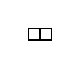
\begin{tikzpicture}[scale=.15]
\draw (0,0) -- (2,0) -- (2,1) -- (0,1) -- cycle (1,0) -- (1,1);
\end{tikzpicture}
}


\begin{document}
\maketitle

\section*{Introduction}

\section{What if squares don't pop?}

\todo{Proposal: split this into a different paper, which aims to describe the braiding, and evaluations of some small knots and polyhedra on the quantum exceptional series. Maybe some should stay here; we're still `above' the exceptional series. --S}

\newcommand{\twosquares}{
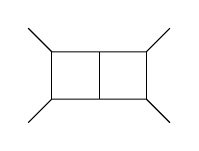
\begin{tikzpicture}[x=0.3cm,y=0.3cm,baseline]
\draw (-3,2) -- (-2,1) -- (2,1) -- (3,2);
\draw (-3,-2) -- (-2,-1) -- (2,-1) -- (3,-2);
\draw (-2,1) -- (-2,-1) (0,1) -- (0,-1) (2,1) -- (2,-1);
\end{tikzpicture}
}
\newcommand{\twosquaresv}{
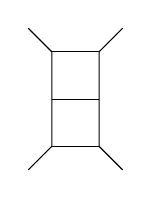
\begin{tikzpicture}[x=0.3cm,y=0.3cm,baseline,rotate=90]
\draw (-3,2) -- (-2,1) -- (2,1) -- (3,2);
\draw (-3,-2) -- (-2,-1) -- (2,-1) -- (3,-2);
\draw (-2,1) -- (-2,-1) (0,1) -- (0,-1) (2,1) -- (2,-1);
\end{tikzpicture}
}


What if we allow the possibility that squares aren't reducible? There are two diagrams  in $D(4,2) \setminus D(4,1)$, namely $$\twosquares \quad \text{ and } \quad \twosquaresv,$$ and so the next interesting possibilities are that there is a relation between these (and lower order terms), so $\dim D(4,2) \leq 6$, or that there are relations simplifying each of these diagrams into lower order terms (i.e. diagrams in $D(4,1)$), so $\dim D(4,1) \leq 5$.

None of the follow results are exhaustive classification statements; they all have additional hypotheses about certain classes of diagrams spanning. Nevertheless, they are interesting because they identify relations that very likely hold in the conjectural (quantum) Vogel plane and (quantum) exceptional series.

We can calculate $M(4,2)$ with entries polynomials in $d, b, t$, the cube $\Cube$, the pentagonal prism $\PentPrism$, the hexagonal prism $\HexPrism$, and the unique polyhedron with four pentagons and four squares $\Q$.

\begin{thm}
$\Delta(4,2) = ...$
\end{thm}

\begin{thm}
One of the follow three possibilities occurs:
\begin{enumerate}
\item The set $D(4,2)$ is linearly independent, and hence $\dim \cC_4 \geq 7$, or 
\item \begin{align*}
\HexPrism & = \frac{\Cube^2 d-\Cube^2-2 \Cube d^2 t^3+2 \Cube d t^3+2 \Cube d t^2-2 \Cube d+d^3 t^6-d^2 \Q t+d^2 \Q-d^2 t^6-3 d^2 t^5+d^2 t^4+4 d^2 t^3-2 d^2 t^2-d^2 t+d^2+d \Q t-2 d \Q}{d (d (-t)+d+t-2)} \\ 
& \twosquares - \twosquaresv =  \alpha_-
 \left( \; 
\drawI
\; - \;
 \drawH
\; \right)
 + \beta_-
\left( \; 
\twostrandid
\; - \;
 \cupcap
\; \right) \\
&\qquad \alpha_- = \\
&\qquad \beta_- =
\end{align*}
or,
\item
\begin{align*}
\HexPrism & = \frac{-\Cube^3 d-\Cube^3-2 \Cube^2 d^2 t^3-2 \Cube^2 d t^3+2 \Cube^2 d t^2+4 \Cube^2 d-\Cube d^3 t^6+\Cube d^2 \Q t+\Cube d^2 \Q+4 \Cube d^2 \PentPrism t^2-\Cube d^2 t^6+\Cube d^2 t^5-5 \Cube d^2 t^4+4 \Cube d^2 t^3-6 \Cube d^2 t^2-\Cube d^2 t-\Cube d^2+\Cube d \Q t+4 \Cube d \PentPrism t^2-4 \Cube d \PentPrism-2 d^3 \Q t^4+4 d^3 \PentPrism t^5+2 d^3 t^8-4 d^3 t^7+6 d^3 t^6-4 d^3 t^5+2 d^3 t^4-2 d^2 \Q t^4+4 d^2 \Q t^2-2 d^2 \Q t-2 d^2 \Q-2 d^2 \PentPrism^2 t-2 d^2 \PentPrism^2+4 d^2 \PentPrism t^5-4 d^2 \PentPrism t^4+4 d^2 \PentPrism t+4 d^2 \PentPrism-2 d \PentPrism^2 t}{d \left(-\Cube d t-\Cube d-\Cube t+2 d^2 t^4+2 d t^4-4 d t^2+2 d t+2 d\right)} \\
& \twosquares + \twosquaresv =  \alpha_+
 \left( \; 
\drawI
\; + \;
 \drawH
\; \right)
 + \beta_+
\left( \; 
\twostrandid
\; + \;
 \cupcap
\; \right) + \gamma_+ \ngon[45]{4} \\
&\qquad \alpha_+ = \\
&\qquad \beta_+ = \\
&\qquad \gamma_+ = 
\end{align*}
\end{enumerate}
\end{thm}
\begin{proof}
Recall that $d+t-dt-2 = 0$ \todo{no! have to separately check the kernel of $M(4,2)$} implies $\cC$ is an $SO(3)_q$ category, and $\dim \cC_4 = 3$. Assuming $d+t-dt-2 \neq 0$, the first component of $\Delta(4,2)$ is exactly the first possibility of the theorem. We find the relation as the kernel of $M(4,2)$. 

If 
\begin{equation*}
\Cube = \frac{2d+2dt-4dt^2+2dt^4+2d^2t^4 }{d+t+dt}
\end{equation*}
then Theorem \ref{thm:cube} applies and $\dim \cC_4 = 4$. Otherwise, and assuming $d+t-dt-2 \neq 0$, the second component of $\Delta(4,2)$ is equivalent to the second possibility of the theorem. Again we find the relation as the kernel of $M(4,2)$. 

\end{proof}

(For those keeping score, Deligne's conjectural exceptional series falls under the first alternative.)

\begin{thm}
If $\dim \cC_4 = 5$ and $D(4,2)$ spans $\cC_4$, 
\begin{equation}
\label{eq:squaresquare}
\twosquares = ...
\end{equation}
\end{thm}
\begin{proof}
Using the previous theorem, we see that it is possible to write $\scalebox{0.4}{\twosquares}$ in terms of $\scalebox{0.4}{\twosquaresv}$ and lower order terms. Thus if $\dim \cC_4 \leq 5$, there must be a relation amongst the diagrams in $D(4,2)$ other than $\scalebox{0.4}{\twosquares}$. Looking at the determinant of corresponding minor of $M(4,2)$, we find
\begin{align*}
\HexPrism & = 
d^{-1} (-dt+d+t-2)^{-1} \left(2 d^2 t^4+2 d t^4-4 d t^2+2 d t+2 d - \Cube (d t+ d+ t)\right)^{-1} \times \\
& \quad \times 
(-\Cube^3 d^2+\Cube^3 d+\Cube^3+3 \Cube^2 d^3 t^4-2 \Cube^2 d^2 t^3-2 \Cube^2 d^2 t^2+4 \Cube^2 d^2-3 \Cube^2 d t^4+2 \Cube^2 d t^3+2 \Cube^2 d t-5 \Cube^2 d-2 \Cube d^4 t^7-\Cube d^4 t^6-2 \Cube d^3 \PentPrism t^3+2 \Cube d^3 \PentPrism t^2+4 \Cube d^3 t^6+8 \Cube d^3 t^5-11 \Cube d^3 t^4+2 \Cube d^3 t^3-\Cube d^3 t^2-\Cube d^3-2 \Cube d^2 \PentPrism t^2+2 \Cube d^2 \PentPrism t-2 \Cube d^2 \PentPrism+2 \Cube d^2 t^7+5 \Cube d^2 t^6-8 \Cube d^2 t^5+\Cube d^2 t^4-2 \Cube d^2 t^3+12 \Cube d^2 t^2-2 \Cube d^2 t-\Cube d^2+2 \Cube d \PentPrism t^3-4 \Cube d \PentPrism t^2-2 \Cube d \PentPrism t+4 \Cube d \PentPrism+d^5 t^{10}-2 d^4 \PentPrism t^6+2 d^4 \PentPrism t^5-4 d^4 t^9+2 d^4 t^8+4 d^4 t^6-4 d^4 t^5+2 d^4 t^4+d^3 \PentPrism^2 t^2-d^3 \PentPrism^2-2 d^3 \PentPrism t^4-2 d^3 \PentPrism t^2+2 d^3 \PentPrism-d^3 t^{10}-2 d^3 t^9-d^3 t^8+16 d^3 t^7-16 d^3 t^6-6 d^3 t^5+8 d^3 t^4+4 d^3 t^3-5 d^3 t^2+d^3+2 d^2 \PentPrism^2+2 d^2 \PentPrism t^6-6 d^2 \PentPrism t^5+4 d^2 \PentPrism t^4+2 d^2 \PentPrism t^2-2 d^2 \PentPrism t-4 d^2 \PentPrism-d \PentPrism^2 t^2+2 d \PentPrism^2 t).
\end{align*}
Substituting this into $\Delta(4,2)$, we obtain $...$, which we can solve for $\Q$ obtaining
\begin{equation*}
\Q = 
d^{-1} (-dt+d+t-2)^{-1} \left(2 d^2 t^4+2 d t^4-4 d t^2+2 d t+2 d - \Cube (d t+ d+ t)\right)^{-1}
(\Cube^3 d^2 t-\Cube^3 t+\Cube^3-\Cube^2 d^3 t^4-2 \Cube^2 d^3 t^3+2 \Cube^2 d^2 t^3+4 \Cube^2 d^2 t^2-4 \Cube^2 d^2 t+\Cube^2 d t^4+4 \Cube^2 d t^3-4 \Cube^2 d t^2+2 \Cube^2 d t-3 \Cube^2 d+3 \Cube d^4 t^7-2 \Cube d^3 \PentPrism t^3+2 \Cube d^3 \PentPrism t^2-4 \Cube d^3 t^6-2 \Cube d^3 t^5+2 \Cube d^3 t^4+8 \Cube d^3 t^3-4 \Cube d^3 t^2-2 \Cube d^2 \PentPrism t^2+2 \Cube d^2 \PentPrism t-2 \Cube d^2 \PentPrism-3 \Cube d^2 t^7-2 \Cube d^2 t^6+\Cube d^2 t^5+13 \Cube d^2 t^4-12 \Cube d^2 t^3-\Cube d^2 t^2+3 \Cube d^2 t+3 \Cube d^2+2 \Cube d \PentPrism t^3-4 \Cube d \PentPrism t^2-2 \Cube d \PentPrism t+4 \Cube d \PentPrism-d^5 t^{10}-2 d^4 \PentPrism t^6+2 d^4 \PentPrism t^5+2 d^4 t^9+4 d^4 t^8-10 d^4 t^7+6 d^4 t^6-2 d^4 t^5+d^3 \PentPrism^2 t^2-d^3 \PentPrism^2-2 d^3 \PentPrism t^4-2 d^3 \PentPrism t^2+2 d^3 \PentPrism+d^3 t^{10}+4 d^3 t^9-7 d^3 t^8-2 d^3 t^7+16 d^3 t^5-12 d^3 t^4-4 d^3 t^3+5 d^3 t^2-d^3+2 d^2 \PentPrism^2+2 d^2 \PentPrism t^6-6 d^2 \PentPrism t^5+4 d^2 \PentPrism t^4+2 d^2 \PentPrism t^2-2 d^2 \PentPrism t-4 d^2 \PentPrism-d \PentPrism^2 t^2+2 d \PentPrism^2 t).
\end{equation*}
Finally, substituting both these values into $M(4,2)$ and computing the kernel, we find the desired relation for $\scalebox{0.4}{\twosquares}$.

\todo{It's not clear to me that it is legitimate to do so, but you can also find this relation as a consequence of both the relations in the previous theorem.}
\end{proof}

To proceed, we introduce some new notation; we use $D^\sqsq(n,k)$ to denote diagrams with $n$ boundary points, at most $k$ internal faces, all of which are at least squares, but with no adjacent squares. We similarly define $M^\sqsq(n,k)$ and $\Delta^\sqsq(n,k)$. We note that $\# D^\sqsq(5,1) = 16$ and $\# D(5,2) = 21$. 

\begin{thm}
Suppose $\dim \cC_4 = 5$ (so the relation of Equation \eqref{eq:squaresquare} holds). Then
$\Delta^\sqsq(5,2) = ...$

Note that this also depends on the value of the associahedron, which has
%the polyhedron p555555444 with 
6 pentagons and 3 isolated squares
$$
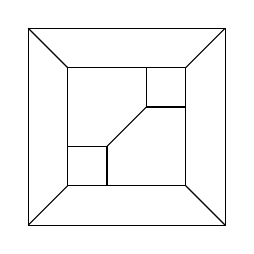
\begin{tikzpicture}[scale=0.5]
\draw (0,0) -- (0,5) -- (5,5) -- (5,0) -- cycle;
\draw (1,1) -- (1,2) -- (2,2) -- (2,1) -- cycle;
\draw (3,3) -- (3,4) -- (4,4) -- (4,3) -- cycle;
\draw (0,0) -- (1,1) (2,2) -- (3,3) (4,4) -- (5,5);
\draw (0,5) -- (1,4) (4,1) -- (5,0);
\draw (1,2) -- (1,4) -- (3,4);
\draw (2,1) -- (4,1) -- (4,3);
\end{tikzpicture}
$$
\end{thm}

\newcommand{\pentasquare}{
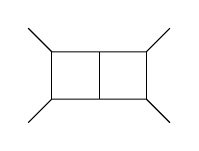
\begin{tikzpicture}[x=0.3cm,y=0.3cm,baseline]
\draw (-3,2) -- (-2,1) -- (2,1) -- (3,2);
\draw (-3,-2) -- (-2,-1) -- (2,-1) -- (3,-2);
\draw (-2,1) -- (-2,-1) (0,1) -- (0,-1) (2,1) -- (2,-1);
\end{tikzpicture}
}


\begin{thm}
Suppose $\cC$ is a trivalent category with $\dim \cC_4=5$ and $\dim \cC_5 = 16$, with $D^\sqsq(5,1)$ a basis for $\cC_5$. \todo{err, with those hypotheses what else could happen?}
Then $\PentPrism$ satisfies a certain degree 6 polynomial (with coefficients rational functions in $d, t,$ and $\Cube$), and there is a relation
\begin{equation*}
pentasquare \in \operatorname{span} D^\sqsq(5,1)
\end{equation*}
with known coefficients in terms of $d, t, \Cube,$ and $\PentPrism$.
\end{thm}
\begin{proof}
The determinant of the 17-by-17 minor of $M^\sqsq(5,2)$ corresponding to the diagrams in $D^\sqsq(5,1)$ along with only one of the 5 rotations of ??? has two(?) irreducible factors.
One is linear in $\PentPrism$, but at the corresponding value of $\PentPrism$ $\Delta^\sqsq(5,1)$ vanishes so $D^\sqsq(5,1)$ cannot be linear independent.
The other is degree 6 in $\PentPrism$, and looking at the kernel of the minor we find the given relation.
\end{proof}

\todo{Does this relation survive inner products with the other pentasquares? I'm hoping that this gives better conditions on $\PentPrism$.  Just take the relation above and apply the 19-by-19 minor to it, and demand that its zero. Hmmm, it seems this gives us the value of 555555444, but no further information about $\PentPrism$. Try $D^\sqsq(5,3)$?}


Next, we introduce $D^{\{\psq,\sqsq\}}(n,k)$, denoting diagrams with $n$ boundary points, at most $k$ internal faces, no adjacent squares, and no square adjacent to a pentagon.

We would like to prove some result about the case $\dim \cC_4 = 5, \dim \cC_5 \leq 16$, $\dim \cC_6 \leq 80$. We see that  $\# D^{\{\psq,\sqsq\}}(6,2) = 80$ and $\# D^{\{\psq,\sqsq\}}(6,3) = 91$, so we hope to identify what happens when $D^{\{\psq,\sqsq\}}(6,2)$ is a basis for $\cC_6$.

\section{Braidings}
To look for a braiding, we want to solve the R2 equation and `sliding a strand over/under a trivalent vertex'. With a pentasquare relation, we can write these equations in a basis.

Does being braided give extra conditions?
What are the values of some small knots?

\section{Sanity checks}
We can compute the values of some small polyhedra for the $14$-dimensional adjoint representation of $(G_2)_q$. As usual, we normalize the trivalent vertex so $b=1$.

\begin{thm}
Taking $X$ to be the $14$-dimensional adjoint representation of $(G_2)_q$, and the trivalent vertex to be the (quantum) Lie bracket normalized so $b=1$, we have

\begin{align*}
d & =  q^{-18} \left(q^{36}+q^{30}+q^{28}+q^{26}+q^{24}+q^{20}+2 q^{18}+q^{16}+q^{12}+q^{10}+q^8+q^6+1\right)\\
t & =\frac{q^2 \left(q^{20}+q^{16}-q^{14}+q^{12}-2 q^{10}+q^8-q^6+q^4+1\right)}{\left(q^2+1\right)^2 \left(q^4-q^2+1\right)^2 \left(q^{12}-q^6+1\right)} \\
\Cube & = \left(q^{36}+q^{30}+q^{28}+q^{26}+q^{24}+q^{20}+2 q^{18}+q^{16}+q^{12}+q^{10}+q^8+q^6+1\right)^5  \times \\
& \quad \times \frac{\left(q^{68}+q^{66}+5 q^{64}+9 q^{62}+13 q^{60}+6 q^{58}+q^{56}-16 q^{54}-26 q^{52}-24 q^{50}+q^{48}+32 q^{46}+57 q^{44}+66 q^{42}+35 q^{40}+2 q^{38}-51 q^{36}-60 q^{34}-51 q^{32}+2 q^{30}+35 q^{28}+66 q^{26}+57 q^{24}+32 q^{22}+q^{20}-24 q^{18}-26 q^{16}-16 q^{14}+q^{12}+6 q^{10}+13 q^8+9 q^6+5 q^4+q^2+1\right)}{q^{24} \left(q^2+1\right)^{12} \left(q^4-q^2+1\right)^{14} \left(q^4+q^2+1\right) \left(q^8-q^4+1\right)^4 \left(q^{12}-q^6+1\right)^7} \\
\PentPrism & = -\left(q^{36}+q^{30}+q^{28}+q^{26}+q^{24}+q^{20}+2 q^{18}+q^{16}+q^{12}+q^{10}+q^8+q^6+1\right)^6 \times \\
& \quad \times \frac{ \left(q^{92}+q^{90}+7 q^{88}+13 q^{86}+30 q^{84}+36 q^{82}+46 q^{80}+4 q^{78}-36 q^{76}-110 q^{74}-112 q^{72}-75 q^{70}+93 q^{68}+260 q^{66}+379 q^{64}+341 q^{62}+90 q^{60}-206 q^{58}-519 q^{56}-478 q^{54}-324 q^{52}+219 q^{50}+505 q^{48}+790 q^{46}+505 q^{44}+219 q^{42}-324 q^{40}-478 q^{38}-519 q^{36}-206 q^{34}+90 q^{32}+341 q^{30}+379 q^{28}+260 q^{26}+93 q^{24}-75 q^{22}-112 q^{20}-110 q^{18}-36 q^{16}+4 q^{14}+46 q^{12}+36 q^{10}+30 q^8+13 q^6+7 q^4+q^2+1\right)}{q^{25} \left(q^2+1\right)^{15} \left(q^4-q^2+1\right)^{18} \left(q^4+q^2+1\right)^2 \left(q^8-q^4+1\right)^5 \left(q^{12}-q^6+1\right)^9}
\end{align*}
\end{thm}


\bibliographystyle{alpha}
\bibliography{../../bibliography/bibliography}


\end{document}
